%version of 04-29-19

\chapter{TECHNIQUES FOR ``DOING'' MATHEMATICS}
\label{ch:doingmath}

\begin{center}
{\it Entia non sunt multiplicanda praeter necessitatem.} \\
\hspace*{3in}{\footnotesize {\bf Occam's Razor}}
\end{center}

\noindent
This famous admonition by William of Occam (14th cent.) to strive for
simplicity is worth heeding when seeking mathematical models of
computational phenomena.

This is the chapter that ``amuses the palate''\footnote{\ldots in the
  sense of the French {\em amuse-bouche}.}~in preparation for the
introductory mathematical repast that we offer the reader.  Before we
present the hors d'oeuvres that we hope will entice the reader, we
``set the table'' for our feast.





Somewhat surprising to the non-mathematician, a large portion of
``doing'' mathematics, the widely touted ``queen of the
sciences''\footnote{See, e.g., Wolfgang Sartorius von Waltershausen,
  {\it Gauss zum Ged\"{a}chtniss} (1856).}, is {\em
  pattern-matching}---albeit of a monumentally sophisticated variety.
Mathematicians are trained to understand pieces of reality to a depth
that allows them to understand how apparently unrelated concepts $A$
and $B$ can be conceptualized via the same abstract representation,
and to analyze (computational, in our bailiwick) advantages to
exploiting such representations.  It may be useful to the reader to
keep the ``mathematics-as-pattern-matching'' metaphor in mind while
reading (from) this book, all the better to enjoy the many instances
of pattern-matching that populate its pages.

This chapter is devoted to the practice of mathematics within the
world of computing.  By means of plentiful examples, we hope to
convince the reader of the importance of mathematics in one's quest
for mastery over the technology and methodology of computing.  By
means of extensive explanations---we often prove the same fact many
times, from multiple, orthogonal vantage points, we hope to provide
the reader with tools for seeing the mathematical aspects of
computational settings and phenomena and technology and with
guidelines for using those tools effectively.

\section{Reasoning via Rigorous Proof}
\label{sec:reasoning-via-proofs}

Mathematics helps one thrive within the world of computing in two
ways: by enabling rigorous argumentation about properties of
computational structures and processes and by enabling cogent analyses
of such properties.  This section is devoted to the first of these
topics.  We survey, explain, and exemplify a range of proof techniques
that are among most commonly useful within computational settings.

\subsection{Classical vs.~modern proofs and methodologies}
\label{sec:classical-v-modern-proofs}

Contrary to the all-too-common view of mathematics as arcane strings
of symbols that must be manipulated in rigid way, mathematics is a
vibrant, evolving system of thinking whose evolution is influenced by
the ever-changing objects that are being thought about and by the
ever-changing population that are doing the thinking.

Gone forever from the world of the practicing mathematician is the
rigidity that characterized the proofs and analyses of the 19th and
early-to-mid-20th century.
\bigskip

\noindent \fbox{
\begin{minipage}{0.95\textwidth}
We do not go back earlier than the 19th century in our quest for
mathmetical proofs because formal notions of rigorous proof are,
historically, a relatively recent phenomenon, stemming largely from
seminal philosophical developments in the 19th century.  Indeed, many
``proofs'' predating the 19th century fall below the standard that
we now expect, even of students.  Indeed, many of what we persist in
calling ``proofs'' from early mathematicians were actually
wrong---even though the theorems were totally correct.
\end{minipage}
}
\bigskip

\noindent
What has replaced the rigid logical systems and rigid prescribed forms
of ``antiquity'' is a vibrant system of thought that, when convenient,
\begin{itemize}
\item
represents the  number $n$, as convenient, by, e.g.,
  \begin{itemize}
  \item
a numeral in some positional number system, such as we use in daily
discourse,
  \item
a set (usually imagined) of $n$ balls or \ldots or widgets,
  \item
a unit-width rectangle that is $n$ units high.
  \end{itemize}

\item
freely uses different modes of argumentation (e.g., numerical and
structural induction, contradiction, counting, \ldots), even mixed and
matched throughout a single analysis;

\item
freely invokes a highly tested computer program to check mind-numbing
proliferations of clerically verifiable details.
\end{itemize}

Regrettably, mathematics education has lagged behind practice, despite
the emergence of technical/technological fields such as computer
science that cannot advance very far without at least informal
extensions and adaptations of the now-archaic formal proof systems.

The current volume is dedicated to trying to overcome people's
resistance to mathematical analysis and argumentation via a modernized
and humanized---but no less rigorous---methodology for ``thinking
mathematically'', especially within computational frameworks.  We
attempt to develop proof systems and methods that the reader can
comfortably develop facility with.

Our avenue for promoting mathematical {\em understanding} rather than
just rote knowledge abjures any specific formalism.  Instead, we
develop multiple proofs for the topics of discourse, involving
multiple representations of the objects being discussed and multiple
modes of argumentation.  The reader will be able to see a variety of
arguments for the same topic, which will hopefully enhance the
likelihood of discovering an approach that is congenial to each
reader's individual way of thinking.  By practicing proofs and
analyses regarding more and more topics, the reader will begin to find
it increasingly easy to state informally what ultimately needs to be
analyzed rigorously and to intuit how to embark on the path toward
such rigor.


\section{The Elements of Rigorous Reasoning}
\label{sec:elements-of-reasoning}

\subsection{Basic Reasoning}

{\em Distinguishing name from object}.
%
A fundamental stumbling block in the road to cogent reasoning arises
from the inability to distinguish names from the objects they denote.
A prime example within the world of computing resides in the inability
to distinguish a function (which can be viewed as an infinite set of
argument-value pairs) from a program, which can be viewed as a name
for the function.  {\bf Note} that the often-used view of a function
as a {\em rule} for assigning values to arguments should be avoided,
because it suggests -- \underline{\em erroneously} -- that an
implementable such rule always exists!

{\em Quantitative reasoning}.
%
Students should understand the foundational distinction between
``growing without bound'' and being innite.  Within this theme, they
should appreciate situations such as the following.  Every integer,
and every polynomial with integer coefficients, is finite, but there
are infinitely many integers and infinitely many polynomials.
Students should be able to verify (cogently but not necessarily via
any particular formalism) assertions such as the following.
\begin{itemize}
\item
Let us be given polynomials $p(x)$ of degree $a$ and $q(x)$ of degree
$b > a$, where $a, b$ need not be integers.  There must exist a
constant $X_{p,q}$ (i.e., a constant that depends on the properties of
polynomials $p$ and $q$) such that for all $x > X_{p,q}$, $p(x) <
q(x)$.

Thus, polynomials having bigger degrees eventually {\em
  majorize}---i.e., have larger values than---polynomials having
smaller degrees.

\item
Continuing with polynomial $q$ of degree $b$: For any real number $c >
1$, there exists a constant $Y_{c;q}$ (i.e., a constant that depends
on the properties of polynomial $q$ and constant $c$) such that for
all $x > Y_{c;q}$, $c^x > q(x)$.

Thus, exponential functions eventually {\em majorize} polynomials.
\end{itemize}

\subsubsection{The Elements of Formal Reasoning}

What is solving mathematical problems?

There are many methods for establishing a formal proof.
In all cases, the problems to solve should be modeled, which means that we 
they are transformed into mathematical problems using formal parameters. 

Then, use techniques like inference, arithmetic operations, induction,
proof by contradiction, etc.

\subsubsection{The Elements of Empirical Reasoning}

Empirical reasoning does not convey the certitude that formal
reasoning does.  


\subsection{What is a ``effective'' proof?}

We are interested in helping the reader learn intuitively compelling,
perspicacious techniques for proving interesting mathematical results.
But what exactly is a ``mathematical proof"---especially within the
context of computational systems and artifacts?  To answer this
question operationally, we follow the lead of the French mathematician
Ren\'e Thom, \index{Thom, Rene\'{e}} the Fields medal winning inventor
of catastrophe theory.  Thom famously defined a proof as an argument
that ``creates a corpus of evidence for educated readers that leads
to their adherence.''
\begin{quote}
{\em Est rigoureuse toute d\'{e}monstration, qui, chez tout lecteur
  suffisamment instruit et pr\'{e}par\'{e}, suscite un \'{e}tat
  d'\'{e}vidence qui entraine l'adh\'{e}sion.}
\end{quote}


\subsubsection{A discussion of ``rigor''}

What to fill in this section?

Historical perspective: Cauchy controversy.

Paper from Leslie Lamport?

TOO COMPLICATED TO PROVE?

\subsubsection{Sample proof}
\label{sec:sample-proofs}


{\Denis Add a simple example here of a typical proof 
with the succession of logical inferences}



\section{Overview of the main proof techniques}

\subsection{Proof by (Finite) Induction}
\label{sec:Induction}

It is crucial that the reader appreciate the fact that proofs by
induction, such as we discuss in this section---and exemplify in
Section~\ref{sec:positive-integer-power}.C---are important tools for
{\em verifying} the correctness of alleged results, but induction by
itself is not a tool for {\em discovering} new results.


\subsubsection{The proof technique}


\subsubsection{Sample proofs: verifying summation formulas}
\label{sec:Proof-Induction}


We illustrate the proof technique of (Finite) Induction by proving the
correctness of two familiar summation formulas: (1) the sum of the
first $n$ positive integers and (2) the sum of the first $n$ odd
positive integers.

\begin{prop}
\label{thm:sum-1-to-n-induction1}
For all $n \in \N$,
\begin{eqnarray}
\nonumber
S_n \ \eqdef \ \sum_{i=1}^n \ i
 & \eqdef &
 1 + 2 + \cdots + (n-1) + n \\
\label{eq:sum-first-n1}
 & = & {1 \over 2} n (n+1) \\
%\nonumber
% & = & {{n+1}  \choose 2}
\end{eqnarray}
\end{prop}

\begin{proof}
For every positive integer $m$, let {\bf P}$(m)$ be the proposition
\[  1 + 2 + \cdot + m \ = \ \frac{m(m+1)}{2} \]
Let us proceed according to the standard format of an inductive
argument.

{\bf 1.} Because $\frac{1(1+1)}{2}  = 1$, proposition {\bf
  P}$(1)$ is true.

{\bf 2.} Let us assume, for the sake of induction, that proposition
{\bf P}$(m)$ is true for all positive integers strictly smaller than
$n$.  In particular, then, {\bf P}$(n-1)$ is true.

{\bf 3.} Consider now the summation
\[ 1 + 2 + \cdots + (n-1) + n \]
Because {\bf P}$(n-1)$ is true, we know that
\[ 1 + 2 + \cdots + (n-1) \ = \ \frac{(n-1)n}{2} \]
By direct calculation, we see that
\begin{eqnarray*}
\frac{(n-1)n}{2} + n
  & = & \frac{n^2 - n + 2n}{2} \\
  & = & \frac{n^2 + n}{2} \\
  & = & \frac{n(n+1)}{2}
\end{eqnarray*}

Because $n$ is an arbitrary positive integer, we conclude that
{\bf P}$(n)$ is true whenever
\begin{itemize}
\item
{\bf P}$(1)$ is true
\item
{\em and}
{\bf P}$(m)$ is true for all $m < n$.
\end{itemize}
By the Principle of (Finite) Induction, then, we conclude that {\bf
  P}$(n)$ is true for all $n \in \N^+$.
\qed
\end{proof}

\bigskip

We turn now to our second summation, which asserts that each perfect
square of a positive integer, say, $n^2$, is the sum of the first $n$
odd integers, $1, 3, 5, \ldots, 2n-1$.  This proof complements the
constructive proofs of the same result in
Proposition~\ref{thm:squares-odd-integers-Gauss}.

\begin{prop}
\label{thm:squares-odd-integers-induction1}
For all $n \in \N^+$,
\[
\sum_{k=1}^n \ (2k-1)
 \ = \ 1 + 3 + 5 + \cdots + (2n-1) \ = \ n^2.
\]
That, is, the $n$th perfect square is the sum of the first $n$ odd
integers.
\end{prop}

\noindent {\em Verification.}
%
For every positive integer $m$, let {\bf P}$(m)$ be the proposition
\[ m^2 \ = \ 1 + 3 + 5 + \cdots + 2m-1. \]
Let us proceed according to the standard format of an inductive
argument.

{\bf 1.} Because $1 \cdot 1 = 1$, proposition {\bf P}$(1)$ is true.

{\bf 2.} Let us assume, for the sake of induction, that proposition
{\bf P}$(m)$ is true for all positive integers strictly smaller than
$n$.  In particular, then, {\bf P}$(n-1)$ is true.

{\bf 3.} Consider now the summation
\[ 1 + 3 + 5 + \cdots + 2n-3 + 2n-1 \]
Because {\bf P}$(n-1)$ is true, we know that
\[ 1 + 3 + 5 + \cdots + 2n-3 + 2n-1 \ = \ (n-1)^2 + 2n-1.  \]
By direct calculation, we see that
\[ (n-1)^2 + 2n-1 \ = \ (n^2 -2n +1) + (2n-1) \ = \ n^2. \]
Because $n$ is an arbitrary positive integer, we conclude that
{\bf P}$(n)$ is true whenever
\begin{itemize}
\item
{\bf P}$(1)$ is true
\item
{\em and}
{\bf P}$(m)$ is true for all $m < n$.
\end{itemize}
By the Principle of (Finite) Induction, then, we conclude that {\bf
  P}$(n)$ is true for all $n \in \N^+$.
\qed



\subsubsection{Making guesses: the method of undetermined coefficients}
\label{sec:undetermined-coefficients1}
\index{method of undetermined coefficients}

Proofs by induction, as provided in
Section~\ref{sec:positive-integer-power}.C, are important tools for
{\em verifying} the correctness of alleged results, but induction by
itself is not a tool for {\em discovering} new results.  This section
is devoted to the {\em Method of Undetermined Coefficients}, a tool
that sometimes yields the ``guesses'' that can then be verified via
induction.  We illustrate the method by deriving a formula for the sum
of the first $n$ perfect squares.  Our derivation builds on prior
knowledge of two facts:
\begin{enumerate}
\item
A trivial proof by counting verifies that
\[ \sum_{k=0}^n \ k^0 \ = \ \sum_{k=1}^n \ 1 \ = \ n.  \]
\item
We know from Proposition~\ref{thm:sum-first-integers-Gauss} that
\[
\sum_{k=0}^n \ k^1 \ = \ \sum_{k=1}^n \ k \ = \ {1 \over 2}(n^2 + n)
\]
\end{enumerate}
\begin{quote}
It seems to be silly to include the case $n=0$ in our summations,
since that term does not affect the sum, but that case tells us that
the ``constant term'' in all of these polynomials---i.e., the
coefficient of $k^0$---is always $c_0 =0$.
\end{quote}

\begin{prop}
\label{thm:sum-of-squares}
For all $n \in \N$,
\begin{eqnarray}
\nonumber
S^{(2)}_n \ \eqdef \ \sum_{i=1}^n \ i^2 
 & \eqdef &
 1 + 4 + \cdots + (n-1)^2 + n^2 \\
\label{eq:sum-1-to-nsq1}
 & = & {1 \over 3} n^3 \ + \ {1 \over 2} n^2 \ + \ {1 \over 6} n
\end{eqnarray}
\end{prop}
\index{formula for the sum of the first $n$ squares}

The target quantity $S^{(2)}_n$ in the proposition is often expressed
in a more aesthetic form:
\[ S^{(2)}_n \ = \
{1 \over 6} n (n+1)(2n+1) \ = \
\frac{2n+1}{3} \cdot {n \choose 2}.
\]

\begin{proof}
Since summing $0$th powers thus gives us a degree-$1$ polynomial, and
summing $1$st powers gives us a degree-$2$ polynomial, it is not
unreasonable to guess that summing $2$nd powers would give us a
degree-$3$ polynomial.  This turns out to be a good guess!  To prove
this assertion, we must determine values for constants $c_1, c_2, c_3$
such that
\begin{equation}
\label{eq:symbolic-cubic1}
\sum_{i=0}^n \ k^2 \ = \ c_3 n^3 + c_2 n^2 + c_1 n.
\end{equation}
(Including the case $n=0$ leaves us with {\em three} constants to
determine rather than four: we know that the coefficient of $k^0$ is
$c_0 =0$.)

We begin our determination of the constants $c_1, c_2, c_3$ by
instantiating the symbolic polynomial in (\ref{eq:symbolic-cubic1}) at
the smallest three values of $n$.  Any three values will work; using
the {\em smallest} ones simplifies our calculations.  These
instantiations leaves us with the following system of linear
equations.  (The summations in (\ref{eq:undetermined}) indicate where
each linear equation in the system comes from.)
\begin{equation}
\label{eq:undetermined}
\begin{array}{lccccccccc}
1. &
{\displaystyle \sum_{i=0}^1 \ k^2}
   & = & c_3    & + & c_2   & + & c_1   & = & 1 \\
2. &
{\displaystyle \sum_{i=0}^2 \ k^2}
   & = & 8 c_3  & + & 4 c_2 & + & 2 c_1 & = & 5 \\
3. &
{\displaystyle \sum_{i=0}^3 \ k^2}
   & = & 27 c_3 & + & 9 c_2 & + & 3 c_1 & = & 14
\end{array}
\end{equation}

We use a form of the {\it Gaussian elimination}
algorithm\footnote{This algorithm is defined and validated in sources
  such as \cite{CLRS}.}~to solve the system by ``eliminating
variables.''  First, we rewrite equation 1 as
\[ 8 c_3 + 8 c_2 + 8 c_1 \ = \ 8 \]
and substract equation 2 from it, thereby obtaining the $2$-variable
equation
\begin{equation}
\label{eq:step1}
4c_2 + 6 c_1 \ = \ 3.
\end{equation}
We perform a similar calculation based on equations 1 and 3 in
system (\ref{eq:undetermined}):  We rewrite equation 1 as
\[ 27 c_3 + 27 c_2 + 27 c_1 \ = \ 27 \]
and substract equation 3 from it, thereby obtaining the $2$-variable
equation
\begin{equation}
\label{eq:step2}
18 c_2 + 24 c_1 \ = \ 13.
\end{equation}
We now rewrite equations (\ref{eq:step1}) and (\ref{eq:step2}) to
obtain the simplified system
\[
\begin{array}{ccccc}
72 c_2 & + & 108 c_1 & = & 54 \\
72 c_2 & + &  96 c_1 & = & 52
\end{array}
\]
We now see, via subtraction, that
\[ 12 c_1 \ = \ 2 \]
or, equivalently,
\begin{equation}
\label{eq:valueof-c1}
c_1 \ = \ 1/6.
\end{equation}

Now that we know the value of $c_1$, we can make the indicated
substitution and further simplify system (\ref{eq:undetermined}).
Since we now have only two variables, we can also eliminate any one
of the three equations in (\ref{eq:undetermined}).  We eliminate
equation 3 in the system in order to simplify our calculations from
this point on.  We now have the system
\begin{equation}
\label{eq:undetermined-step2}
\begin{array}{lccccc}
1. &
c_3  & + & c_2   & = & 5/6 \\
2. &
8c_3 & + & 4 c_2 & = & 14/3 
\end{array}
\end{equation}
We rewrite equation 1 in (\ref{eq:undetermined-step2}) as
\[ 8 c_3 + 8 c_2 \ = \ 20/3 \]
and subtract equation 2 from this version of equation 1.  We thereby
discover that
\[ 4 c_2 \ = \ 2, \]
or, equivalently,
\begin{equation}
\label{eq:valueof-c2}
c_2 \ = \ 1/2.
\end{equation}

Using the values we have discovered for $c_1$ and $c_2$, in equations
(\ref{eq:valueof-c1}) and (\ref{eq:valueof-c2}), respectively, we
finally use equation 1 of system (\ref{eq:undetermined}) to determine
the value of $c_3$:
\begin{equation}
\label{eq:valueof-c3}
c_3 \ = \ 1 - \ 1/2 \ - \ 1/6 \ = \ 1/3.
\end{equation}
We have, thus, derived equation~(\ref{eq:sum-1-to-nsq1}).

\medskip

The careful reader will note that we are not really done yet.  We
have derived our expression for $S^{(2)}_n$ under the as-yet
unjustified assumption that $S^{(2)}_n$ really is a cubic (i.e.,
degree-$3$) polynomial.  What we need now is an induction that will
verify our result.  With our previous illustrations as models, we
shall leave this final task to the reader.

\qed
\end{proof}

With more (calculational) work, but no new (mathematical) ideas, one
can derive explicit expressions for the sum of the first $n$ $k$th
powers, i.e., the quantity $S^{(k)}_n$, for any positive integer $k$.


\subsection{Proof by Contradiction}
\label{sec:Contradiction}
\index{proof by contradiction}

\begin{quote}
{\em The importance of this proof technique has been recognized since
  antiquity, under the Latin names {\em contradictio in contrarium}
  and, perhaps less accurately, {\em reductio ad absurdum}.}
\end{quote}



\subsubsection{The Proof Technique}
\label{sec:contradiction-technique}
\index{proof by contradiction!technique}



The basic principle that underlies proof by contradiction is that the
following {\em metamathematical} assertions are logically equivalent.
\begin{itemize}
\item
Proposition $P$ {\sc implies} Proposition $Q$
\item
Proposition $\sim Q$ {\sc implies} Proposition $\sim P$
\end{itemize}

As with many of these {\em metamathematical} principles, there is a
corresponding {\em mathematical} equivalence, in this case,
Proposition~\ref{thm:contraposition}.
\[ [P \Rightarrow Q] \ \equiv \ [(\sim Q) \Rightarrow (\sim P)] \]


\subsubsection{Sample Proofs}
\label{sec:sample-contradictions}
\index{proof by contradiction!sample proofs}

\paragraph{\small\sf A. There are infinitely many primes}

The following result is traditionally attributed to the Greek
mathematician Euclid,
\index{Euclid}
one of the patriarchs of mathematics.

\begin{prop}
\label{thm:Primes-infinite}
There are infinitely many prime numbers.
\end{prop}

\begin{proof}
Let us assume, contrarily, that there are only finitely many primes.
Say, in particular, that the following $r$-element sequence enumerates
all (and only) primes, in order of magnitude:

$\mbox{\bf Prime-Numbers} \ = \ 
\langle P_1, \ P_2, \ \ldots, \ P_r \rangle$

\noindent where
\begin{itemize}
\item
$P_1 = 2$
\item
$P_2 = 3$
\item
$P_i < P_{i+1}$ for all $i \in \{1, 2, \ldots, r-1\}$.
\end{itemize}

We verify the {\em falseness} of the alleged completeness of the sequence
{\bf Prime-Numbers} by analyzing the positive integer
\[ n \ = \ 1 + \prod_{i=1}^r \ P_i \ = \ 1 \ + \ 
\left(P_1 \cdot P_2 \cdot \cdots \cdot P_r \right).
\]

We make three crucial observations.

\begin{enumerate}
\item
We note first that {\em the number $n$ is not divisible by any prime
number  in the sequence {\bf Prime-Numbers}.}

To see this, note that for each $P_k$ in the sequence,
\[
n / P_k \ = \ \frac{1}{P_k} \ + \ \prod_{i \neq k} \ P_i .
\]
Because $P_k \geq 2$, we see that $n / P_k$ obeys the inequalities
\[
\prod_{i \neq k} \ P_i \ < \ n/P_k \ < \ 1 + \prod_{i \neq k} \ P_i.
\] 
The discreteness of the set $\Z$---see
Section~\ref{sec:integers}.A---implies that $n / P_k$ is not an
integer, because it lies strictly between two adjacent integers.

\item
We note next that, because of assertion 1, if the sequence {\bf
  Prime-Numbers} actually contained {\em all} of the prime numbers,
then we would have to conclude that {\em the number $n$ is not
  divisible by any prime number.}

\item
Finally, we remark that the Fundamental Theorem of Arithmetic
(Theorem~\ref{thm:Fund-Thm-Arith}) implies that {\em every integer is
  divisible by (at least one) prime number}.
\end{enumerate}

We have a chain of assertions that lead to a mutual inconsistency: on
the one hand, the integer $n$ has no prime-integer divisor; on the
other hand, no integer can fail to have a prime-integer divisor!  Let
us analyze how we arrived at this uncomfortable place.
\begin{itemize}
\item
At the front end of this uncomfortable string of assertions we have
the assumption that there are only finitely many prime numbers.  We
have (as yet) no substantiation for this assertion.
\item
At the back end of this uncomfortable string of assertions we have
the ({\em rock solid}) Fundamental Theorem of Arithmetic
(Theorem~\ref{thm:Fund-Thm-Arith}).
\item
In between these two assertions we have a sequence of assertions, each
of which follows from its predecessors via irrefutable rules of
inference.
\end{itemize}
It follows that the {\em only} brick in this edifice that could be
faulty---i.e., the only assertion that could be false---is the
assumption that there are only finitely many prime numbers.  Since
this assumption leads to an inconsistent set of assertions, we must
conclude that the assumption is false!  We conclude from this
classical proof by contradiction that there are infinitely many prime
numbers.  \qed
\end{proof}



\subsection{Geometrical and graphical proofs}
\label{sec:unconventionalproofs}

\subsubsection{When geometry raised}

Quotation from Plato
\textit{Que nul n'entre ici s'il n'est g\'eom\`etre}
\medskip

We present below a very simple example of a \textit{geometrical} proof, 
which consists in solving a problem by an analogy with basic geometrical objects
(here the surfaces of square and rectangles). 
Let consider the following equation:
\begin{equation}
(n+1)^2 \ = \ n^2 \ + \ 2n \ + \ 1.
\end{equation}

This result can also be established using the highly perspicuous
Fig.~\ref{fig:proofa2plusb2}.
%{\Denis We can remark here that this result is straightforward as
%follows. see below if you think it should be included.}
\begin{figure}[ht]
\begin{center}
       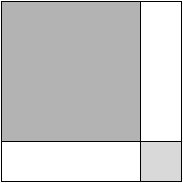
\includegraphics[scale=0.4]{FiguresMaths/proofa2plusb2}
\caption{A geometrical proof of the identity $(n+1)^2 = n^2 + 2n + 1$.}
       \label{fig:proofa2plusb2}
\end{center}
\end{figure}
The figure tells its tale by exhibiting four rectangles that make up
an $(n+1) \times (n+1)$ square; the area of this square is, of course,
$(n+1)^2$.  This large square is made up of four rectangles.
\begin{itemize}
\item
Reading across the top of the figure, we encounter a darkly shaded $n
\times n$ square (area $= n^2$) and an unshaded $n \times 1$ rectangle
(area $= n$).
\item
Reading across the bottom of the figure, we encounter an unshaded $1
\times n$ rectangle (area $= n$) and a lightly shaded $1 \times 1$
square (area = $1$).
\end{itemize}
The overall message is that $(n+1)^2$ (the area of the large,
composite, square)

\begin{tabular}{ll}
is the sum of & \\
  & $n^2$ (the area of the darkly shaded square) \\
plus & \\
  & $2n$ (the combined areas of the unshaded rectangles) \\
plus & \\
  & $1$ (the area of the lightly shaded square)
\end{tabular}


\subsubsection{Fubini's principle}
\label{sec:Fubini}

Give the definition and describe the principle here

Let us illustrates this type of proof on the problem of computing the sum of the $n$ first integers.


\index{Fubini, Guido}


\subsection{Proofs via the Pigeonhole Principle}
\label{sec:pigeonhole}

{\Denis Is it a technique by itself like the other ones or should it be integrated into another one -- on thus, which one?}

The proof technique we discuss now builds on an observation that is
almost embarrassingly obvious---yet its simplicity is exceeded by its
importance as a source of strikingly surprising results.

\subsubsection{The Proof Technique}

The technique, known variously as {\it the pigeonhole principle}
\index{pigeonhole principle}
or {\it Dirichlet's Box Principle}
\index{Dirichlet's Box Principle}
(after the French mathematician Peter Gustav Lejeune Dirichlet),
\index{Dirichlet, Peter Gustav Lejeune}
exploits the fact that if one has $n$ objects (say, pigeons) and $m <
n$ boxes (they're the pigeonholes), then any way of putting pigeons
into boxes must place at least two pigeons into the same box.


\subsubsection{Sample (Fun) Applications/Proofs}
\label{sec:pigeon-apps}


\paragraph{\small\sf Choosing a pair of matching socks} 

You have $n$ pairs of socks, the socks in each pair having a distinct
color (one pair of red socks, one pair of blue socks, \ldots).  Since
you wake up ``very slowly'', you want to grab some number of unpaired
socks that is certain to yield at least one pair of same-color socks.
Clearly, if you grab any $n+1$ socks (the pigeons), the pigeonhole
principle guarantees that you have at least one monochromatic pair,
because there are only $n$ distinct sock-colors (the boxes).


\ignore{
\paragraph{\small\sf B. Finding birthday-mates}

You are attending a conference and wander into a lecture that has 367
attendees (including you).  It is certain that at least two attendees
share the same birthday: there are 366 possible birthdays (the boxes
for a leap year) and 367 birthday-possessors (the pigeons).

{\Denis May be we can put this in exercice and add the anniversary paradox which state a similar question with probabilities?}
}

\paragraph{\small\sf Friends and strangers at a party}

We turn now to a somewhat more surprising result that can be proved
using the pigeonhole principle.  While we phrase the result in
anthropomorphic, ``homely'', terms, its formal statement identifies it
as a genre of ``unavoidable subgraph''
\index{unavoidable subgraph phenomena}
%
phenomenon within the theory of {\it graphs}.
\begin{quote}
Graphs are an immensely important mathematical construct that models
myriad situations that involve objects (possibly people) and
interrelationships between pairs of objects.
Chapter~\ref{ch:Graphs-Trees} is devoted to studying graphs and the
situations they can be used to model---including the problem discussed
here.
\end{quote}
Here is the ``homely'' version of the {\it Friends and Strangers} problem.
\index{friends and strangers problem}

\begin{prop}
\label{thm:triangle-cotriangles}
In any gathering of six people, at least one of the following
assertions is true.

\noindent {\rm A.}
There is a group of three people who know each other.

\noindent {\rm B.}
There is a group of three people none of whom knows either of the
others.
\end{prop}

\begin{proof}
Let the gathering consist of six indistinguishable people, named
$P_1$, $P_2$, $P_3$, $P_4$, $P_5$, $P_6$.  Focus on an arbitrary
person, say $P_5$.  (This choice ``sounds'' more arbitrary than
$P_1$---but, of course, is not.)  Now, there are $5$ people, namely,
$P_1$, $P_2$, $P_3$, $P_4$, $P_6$, each of whom $P_5$ either {\em
  knows} or {\em doesn't know}.

Clearly, some $3$ of these $5$ people ``lie on the same side of the
{\em know/don't-know} fence.''  This follows from the pigeonhole
principle: we have {\em two} boxes ({\em know} and {\em doesn't know})
and {\em five} pigeons (the people $P_1$, $P_2$, $P_3$, $P_4$, $P_6$).
Any way of putting the pigeons into the boxes will place three people
into one of the boxes.

Say, with no loss of generality, that $P_5$ {\em knows} $P_1$, $P_2$,
$P_3$.
\begin{quote}\index{``with no loss of generality'': meaning}
Why can we claim that the selected situation--- ``$P_5$ {\em knows}
$P_1$, $P_2$, $P_3$''---can be assumed ``with no loss of generality''?
One should {\em always} ask this question about such a claim!  In the
current case, the claim follows from the following facts.

(a) The names that we use to refer to the six assembled people are
just for our expository benefit.  The names carry no inherent meaning
related to the {\it Friends and Strangers} problem.  You can repeat
our argument while choosing arbitrary replacements for $P_1$, $P_2$,
$P_3$, $P_5$, with no change to the logical outcome.

You can also interchange the {\em know} and {\em don't-know} labels.
The underlying logic will not change, although the conclusions
regarding options A and B in the statement of the proposition will
clearly ``flip''.
\end{quote}

Having decided that $P_5$ {\em knows} $P_1$, $P_2$, and $P_3$, we now
consider the implications of the possible relations between each of
the three pairs of people chosen from $\{P_1, P_2, P_3\}$.  There
are two logical possibilities.
\begin{itemize}
\item
Some two of $P_1$, $P_2$, $P_3$ know each other---say, with no loss of
generality, $P_1$ and $P_2$.  In this case, $P_1$, $P_2$, and $P_5$
form a trio of people who know one another (option A in the statement
of the proposition).
\item
No two of $P_1$, $P_2$, $P_3$ know each other.  In this case, $P_1$,
$P_2$, and $P_3$ form a trio of people none of whom knows either of
the others (option B in the statement of the proposition).
\end{itemize}
This disjunction completes the proof.

We close the proof by noting that nothing we have stated precludes the
possibility that {\em both} option A {\em and} option B are true!  \qed
\end{proof}


\subsection{Combinatorial Proofs}

We introduce here a less conventional type of proofs that look at a result
as counting using combinatorial arguments.
This is illustrated by the previous example of computing the sum of the $n$ first integers:
\[ 1+2+ \ldots + n \ = \ {n \choose 2}.  \]
Choosing $2$ elements among $n$ can be done by choosing the last element (say at index $k$)
{\Denis k starts at 2 and goes to n}
and then, choosing the other one among the $k-1$ remaining ones before $k$, 
which can be mathematically written as:
\[ \ {n \choose 2} \ = \  \sum_{k=2}^n  \ {k-1 \choose 1} \ = \  \sum_{k=2}^n  (k-1) \ = \  \sum_{k=1}^{n-1}  k \ = \ \frac{(n)(n-1)}{2}\]


\subsection{Reasoning via Mathematical Analysis}
\label{sec:analysis}

{\Denis I am not clear about this section.
What should it contain?}


\subsection{Proof by computer}

{\Denis I suggest here to include a word about the proof by computer, tell the story of 
the 4-color theorem.}

%\subsection{Analyses via Linear Recurrences}
%\label{sec:linear-recurrences-1}
%
%\begin{theorem}[The Master Theorem for Linear Recurrences]
%\label{thm:master-thm-1}
%\index{The Master Theorem for Linear Recurrences}
%Let the function $F$ be specified by the following linear recurrence.
%\begin{equation}
%\label{eq:Lin-Recur:start-1}
%F(n) \ = \ \left\{
%\begin{array}{cl}
%a F(n/b) + c & \mbox{for } n \geq b \\
%c & \mbox{for } n < b
%\end{array}
%\right.
%\end{equation}
%Then the value of $F$ on any argument $n$ is given by
%\begin{equation}
%\label{eq:Lin-Recur:solve-1}
%\begin{array}{lclll}
%F(n) & = & (1 + \log_b n)c &  & \mbox{if } a=1 \\
%     &   &                 &  & \\
%     & = &
%  {\displaystyle
%  \frac{1-a^{\log_b n}}{1-a} \ \approx \ \frac{1}{1-a}
%  }
% &  & \mbox{if } a<1 \\
%    &   &                  & & \\
%    & = &
%  {\displaystyle
%\frac{a^{\log_b n} -1}{a-1}
%  }
% & & \mbox{if } a>1
%\end{array}
%\end{equation}
%\end{theorem}
%
%


